%%%% CAPÍTULO 2 - REVISÃO DA LITERATURA (OU REVISÃO BIBLIOGRÁFICA, ESTADO DA ARTE, ESTADO DO CONHECIMENTO)
%%
%% O autor deve registrar seu conhecimento sobre a
%% literatura básica do assunto, discutindo e 
%% comentando a informação já publicada. A revisão deve
%% ser apresentada, preferencialmente, em ordem
%% cronológica e por blocos de assunto, procurando
%% mostrar a evolução do tema.

%% Título e rótulo de capítulo (rótulos não devem conter caracteres especiais, acentuados ou cedilha)
\chapter{Revisão da Literatura}\label{cap:revisaodaliteratura}

\section{Trabalhos relacionados} \label{sec:fund}

\textcolor{courb2020}{
Para análise de desempenho da operação do transporte, é necessário incluir informação de tempo no modelo de rede utilizado. Em \cite{hol:12}, uma variedade de termos é apresentada para designar redes cuja estrutura é dependente do tempo: \emph{temporal graphs}, \emph{evolving graphs}, \emph{time-varying graphs}, \emph{time-aggregated graphs}, \emph{time-stamped graphs}, \emph{dynamic networks}, \emph{dynamic graphs}, \emph{dynamical graphs}, entre outros. O objetivo aqui não é discutir estes termos em profundidade, mas apenas destacar a ampla gama de opções para modelagem de redes dinâmicas. Particularmente, o modelo \emph{Time Varying Graph} (TVG) é adotado neste trabalho, tendo sido usado em \cite{sant:09}, além de \cite{tang:10} e \cite{lat:10} como uma sequência discreta e ordenada de grafos (a forma mais intuitiva de representação de um grafo variante no tempo). Um extensão dos conceitos clássicos de grafos para TVGs é apresentada em \cite{lat:12}. Em \cite{wach:19}, é apresentado um modelo TVG do transporte de ônibus de Greater Moncton no Canadá e sua implementação no banco de dados de grafos Neo4j\footnote{http://neo4j.org}. Conforme apontado em \cite{vick:10}, há um interesse crescente em bancos de dados noSQL (\emph{not only} SQL), como o Neo4j, para armazenamento e recuperação de dados com informação dinâmica.
}


\section{Grafos} \label{sec:fund}

A  Figura~\ref{fig:graphtheory}

 \begin{figure}[!h]
 \caption{Origem da teoria dos grafos}
     \centering
     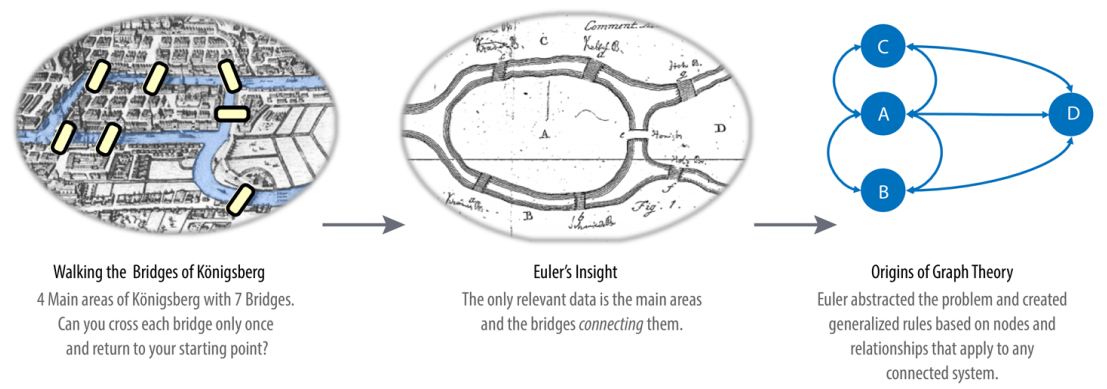
\includegraphics[scale=.40]{./Capitulo2/img/origins-graph-theory.png}
         \label{fig:graphtheory}
     \fonte{\cite{needham:2019}}
 \end{figure}
 
 
\section{Time Varying Graph (TVG)} \label{sec:fund}

%Referências:\\
%\cite{hol:12} (Mais geral sobre Temporal Networks; Samaki tem )\\
%\cite{lat:10} (Menciona TVGs como uma sequência de grafos)\\
%\cite{sant:12} (TVG basico)\\
%\cite{cat:13} (TVG e Neo4j)\\
%\cite{lat:12} (TVG)\\
%\cite{wach:17} (People in Motion Lab)\\
%\cite{wach:19} (People in Motion Lab)\\
%\cite{vick:10} (Comparação Graph and Relational Database)
\textcolor{courb2020}{
O termo \emph{Time Varying Graph} (grafo variante no tempo ou TVG) pode ser encontrado em \cite{sant:09}, \cite{tang:10}, \cite{lat:10} e \cite{lat:12}. O formalismo adotado no presente trabalho é devido a~\cite{sant:12}. 
}
\textcolor{courb2020}{
Um TVG é uma quíntupla $\mathcal{G}=(V,E,\mathcal{T},\rho,\zeta)$, tal que $V$ e $E$ são os conjuntos de vértices e arestas do grafo rotuladas pelo conjunto $L$ de rótulos ($E \subseteq V \times V \times L$), respectivamente, $\mathcal{T}\subseteq \mathbb{T}$ é o tempo de vida do sistema, $\rho: E \times \mathcal{T} \rightarrow \{0,1\}$ é a função de presença e $\zeta: E \times \mathcal{T} \rightarrow \mathbb{T}$ é a função de latência. O domínio temporal $\mathbb{T}$ é assumido igual a $\mathbb{N}$ para sistemas a tempo discreto e $\mathbb{R}^+$ para para sistemas a tempo contínuo.
}
\textcolor{courb2020}{
A função $\rho$ indica a presença (1) ou não (0) de uma aresta em um determinado instante de tempo e a função $\zeta$ representa o tempo necessário para cruzar uma aresta a partir de um determinado instante de tempo (a latência pode variar com o tempo). Este modelo é geral o suficiente para representar vários cenários, desde redes de comunicação e transporte até sistemas complexos ou redes sociais~\cite{sant:12}. 
}
\textcolor{courb2020}{
Por exemplo, um TVG pode ser usado para modelar viagens de uma cidade $A$ para uma cidade $B$. As cidades $A$ e $B$ são os vértices do grafo conectados por duas arestas paralelas rotuladas `ônibus' e `carro' para indicar viagens feitas de ônibus e de carro, respectivamente. Neste caso, a viagem de ônibus inicia em instantes de tempo determinados e, portanto, a função $\rho$ da aresta `ônibus' retorna valor 1 apenas nas datas e horários para os quais a viagem de ônibus pode ser iniciada. A função de latência $\zeta$ de cada aresta  pode retornar diferentes valores, dependendo dos tempos de viagem de ônibus e de carro (ou mesmo diferentes valores para uma mesma aresta, dependendo do tempo de viagem em diferentes horários).
}
\textcolor{courb2020}{
A partir deste modelo geral de~\cite{sant:12}, um modelo de dados é proposto em \cite{cat:13} para capturar o comportamento temporal de redes sociais e implementado no banco de dados de grafos Neo4j. O banco Neo4j implementa um tipo de grafo denominado \emph{property graph model}, capaz de representar multigrafos direcionados, rotulados e com atributos. Estes grafos permitem a representação de vértices e arestas rotulados, além de metadados (propriedades) associados aos vértices e arestas~\cite{rod:10}, particularmente importantes na implementação de TVGs. Além disso, o banco de dados Neo4j tem outras características que favorecem a implementação: (i) armazenamento persistente e transacional de grafos de elevada dimensão; suporte para análise em profundidade via buscas eficientes de múltiplos saltos; (iii) suporte para linguagem declarativa de \emph{queries} de grafos denominada Cypher\footnote{https://neo4j.com/docs/cypher-manual/current/}.
}
\textcolor{courb2020}{
O modelo proposto para o transporte público de Curitiba tem por base o modelo de grafo utilizado em \cite{wach:19} para o transporte de ônibus da região de Greater Moncton no Canadá. Este modelo deriva de~\cite{cat:13}, tendo sido também implementado no banco Neo4j.
}

